%!TEX root = ..\MainFile.tex
\section{Компьютерные модели групповой динамики} % (fold)
\label{sec:ComputerModelsOfHords}

\epigraph{Позабыты~хлопоты,~остановлен~бег~- \\
Вкалывают роботы, а не человек.}{Ю. Энтин - ``Вкалывают роботы''}
Как было сказано в разделе \ref{sec:AnimalFlocking}, основной сложностью в исследовании процессов, происходящих в рое является невозможность уследить сразу за всеми представителями. В первую очередь проблема заключается в высокой технической сложности гарантированно отличить одну особь от другой.

            \subsection{Компьютерные модели групповой динамики} % (fold)
            \label{sub:CompModelsCollMot}
            Моделированием групповых эффектов начали заниматься в 70е годы несколько групп ученых - биологов, физиков и специалистов по коспьютерной графике. 
            \begin{figure}
                \centering
                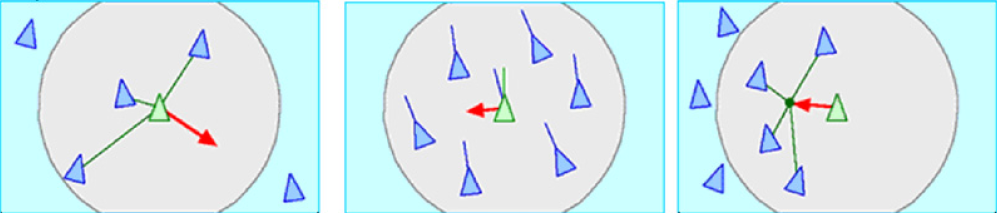
\includegraphics[width=\textwidth]{Fig31_CollectiveMotion}
                \caption{Поведение, основное для модели Рейнольдса. (а) Разделение, с тем чтобы избежать чрезмерного скапливания боидов. (б) Выравнивание: боиды поворачивают в направлении средней скорости окружающих боидов. (в) Когезия: боиды смещаюстся в направлении центра масс окружения}
                \label{fig:ReynoldsModel}
            \end{figure}
            Первая широко известная модель была предложена Рейнольдсом \cite{reynolds1987}. В его модели поведение обьектов (боидов) определялось из рассчета наилучшего визуального представления. Боиды могли демонстрировать три типа взаимодействия - избегание столкновений, следование в направлении ближайших боидов, и стремление к центру масс стаи. \ref{fig:ReynoldsModel} С тем чтобы привнести в изучение групповых эффектов количественный подход, была предложена модель, широко известная сейчас как ``модель Вичека'' \cite{vicsek1995}. Поведение частиц в этой модели определяется следующими соотношениями:
            \begin{equation}
                \vec{v}_i(t+1) = v_0 \frac{{\langle \vec{v}_i(t) \rangle}_R}{|{\langle \vec{v_j}(t) \rangle}_R|} + perturbation
            \end{equation}
            \begin{equation}
                \vec{x}_i(t+1) = \vec{x}_i(t)+\vec{v}_i(t+1)
            \end{equation}
            Здесь ${\langle \dots \rangle}_R$ обозначают усреднение (или суммирование) по всем частицам в радиусе $R$ вокруг $i$-й. Тогда $ \frac{{\langle \vec{v}_i(t) \rangle}_R}{|{\langle \vec{v_j}(t) \rangle}_R|}$ предоставляет нам единичный вектор в направлении средней скорости группы частиц. Такое выравнивающее правило не принимает во внимание характер взаимодействия, и потому модель может соответствовать когезии, взякости и тому подобному. Введение шума в модель может выполняться различными способами. В оригинальной работе было предложено следующее: поскольку единичный вектор однозначно соответствует углу, задающему направление, и скорость частиц также можно задавать в виде модуля скорости и единичного вектора направления, то тогда угол направления движения в момент времени $(t+1)$ получается следующим образом:
            \begin{equation}
                \vartheta_i (t+1) = \vartheta_i(t) + \Delta_i(t)
            \end{equation}
            где $\vartheta_i(t) = \arctan [{\frac{{\langle \vec{v}_i(t) \rangle}_R}{|{\langle \vec{v_j}(t) \rangle}_R|}}]$, и шум представлен $\Delta_i(t)$ - случайное число равновероятно выбранное из $[-\eta \pi,\eta \pi]$. Единственными параметрами модели является плотность $\rho$, модуль скорости частиц $v_0$ и уровень шума, определяемый $\eta < 1$. Параметром порядка становится 
            $\varphi = 1/{N v_0} |{\sum\limits_{i=1}^n \vec{v_i}}|$, как определно в уравнени \ref{eq:OrederParam}.

            Несмотря на кажущуюся простоту этой модели, она демонстрирует богатый спектр свойств, характерных для систем, демонстрирующих групповую динамику. В первую очередь это конечно же фазовый переход к упорядоченному движению. Помимо этого, варьируя указанные выше параметры модели, удавалось получить различные паттерны
            % subsection CompModelsCollMot (end)

% section section_name (end)